\documentclass[10pt]{article}
\usepackage[paperwidth=30cm,paperheight=21cm,margin=0.9cm]{geometry}
\usepackage[T1]{fontenc}
\usepackage{lmodern}
\usepackage{amsmath,amssymb}
\usepackage{tikz}
\usetikzlibrary{arrows.meta,calc,positioning,backgrounds}
\pagestyle{empty}
\setlength{\parindent}{0pt}
\renewcommand{\familydefault}{\sfdefault}

\definecolor{ink}{HTML}{183047}
\definecolor{fixed}{HTML}{536779}
\definecolor{fixedbg}{HTML}{F0F4F7}
\definecolor{learned}{HTML}{006D77}
\definecolor{learnedbg}{HTML}{E8F5F3}
\definecolor{task}{HTML}{365DA8}
\definecolor{taskbg}{HTML}{EDF2FC}
\definecolor{heldout}{HTML}{9C6723}
\definecolor{heldoutbg}{HTML}{FFF4E3}

\tikzset{
  box/.style={draw=fixed!70,fill=fixedbg,rounded corners=2mm,
    line width=0.65pt,align=center,inner sep=5pt,font=\small,text=ink},
  fixedbox/.style={box},
  learnedbox/.style={box,draw=learned,fill=learnedbg},
  taskbox/.style={box,draw=task,fill=taskbg},
  testbox/.style={box,draw=heldout,fill=heldoutbg},
  flow/.style={-{Stealth[length=2.1mm,width=1.5mm]},draw=ink,line width=0.85pt},
  gradient/.style={flow,draw=learned,dashed,line width=1pt},
  label/.style={font=\scriptsize,text=ink,align=center,fill=white,inner sep=2pt},
  section/.style={font=\bfseries\small,text=ink,anchor=west},
  panel/.style={draw=fixed!25,rounded corners=2.5mm,line width=0.6pt,fill=white},
}

\newcommand{\heading}[2]{%
  {\LARGE\bfseries\color{ink}#1}\par\vspace{2mm}
  {\small\color{fixed}#2}\par\vspace{2mm}}

\begin{document}
\heading{MouseLFP: current network architecture}{%
  Fixed spectral basis \(\longrightarrow\) shared residual frontend
  \(\longrightarrow\) task-local CNN. Shapes include batch size \(B\).}
\begin{center}
% Shape conventions: Conv2d = B,C,T,F; CNN input = B,C,E,T,F.
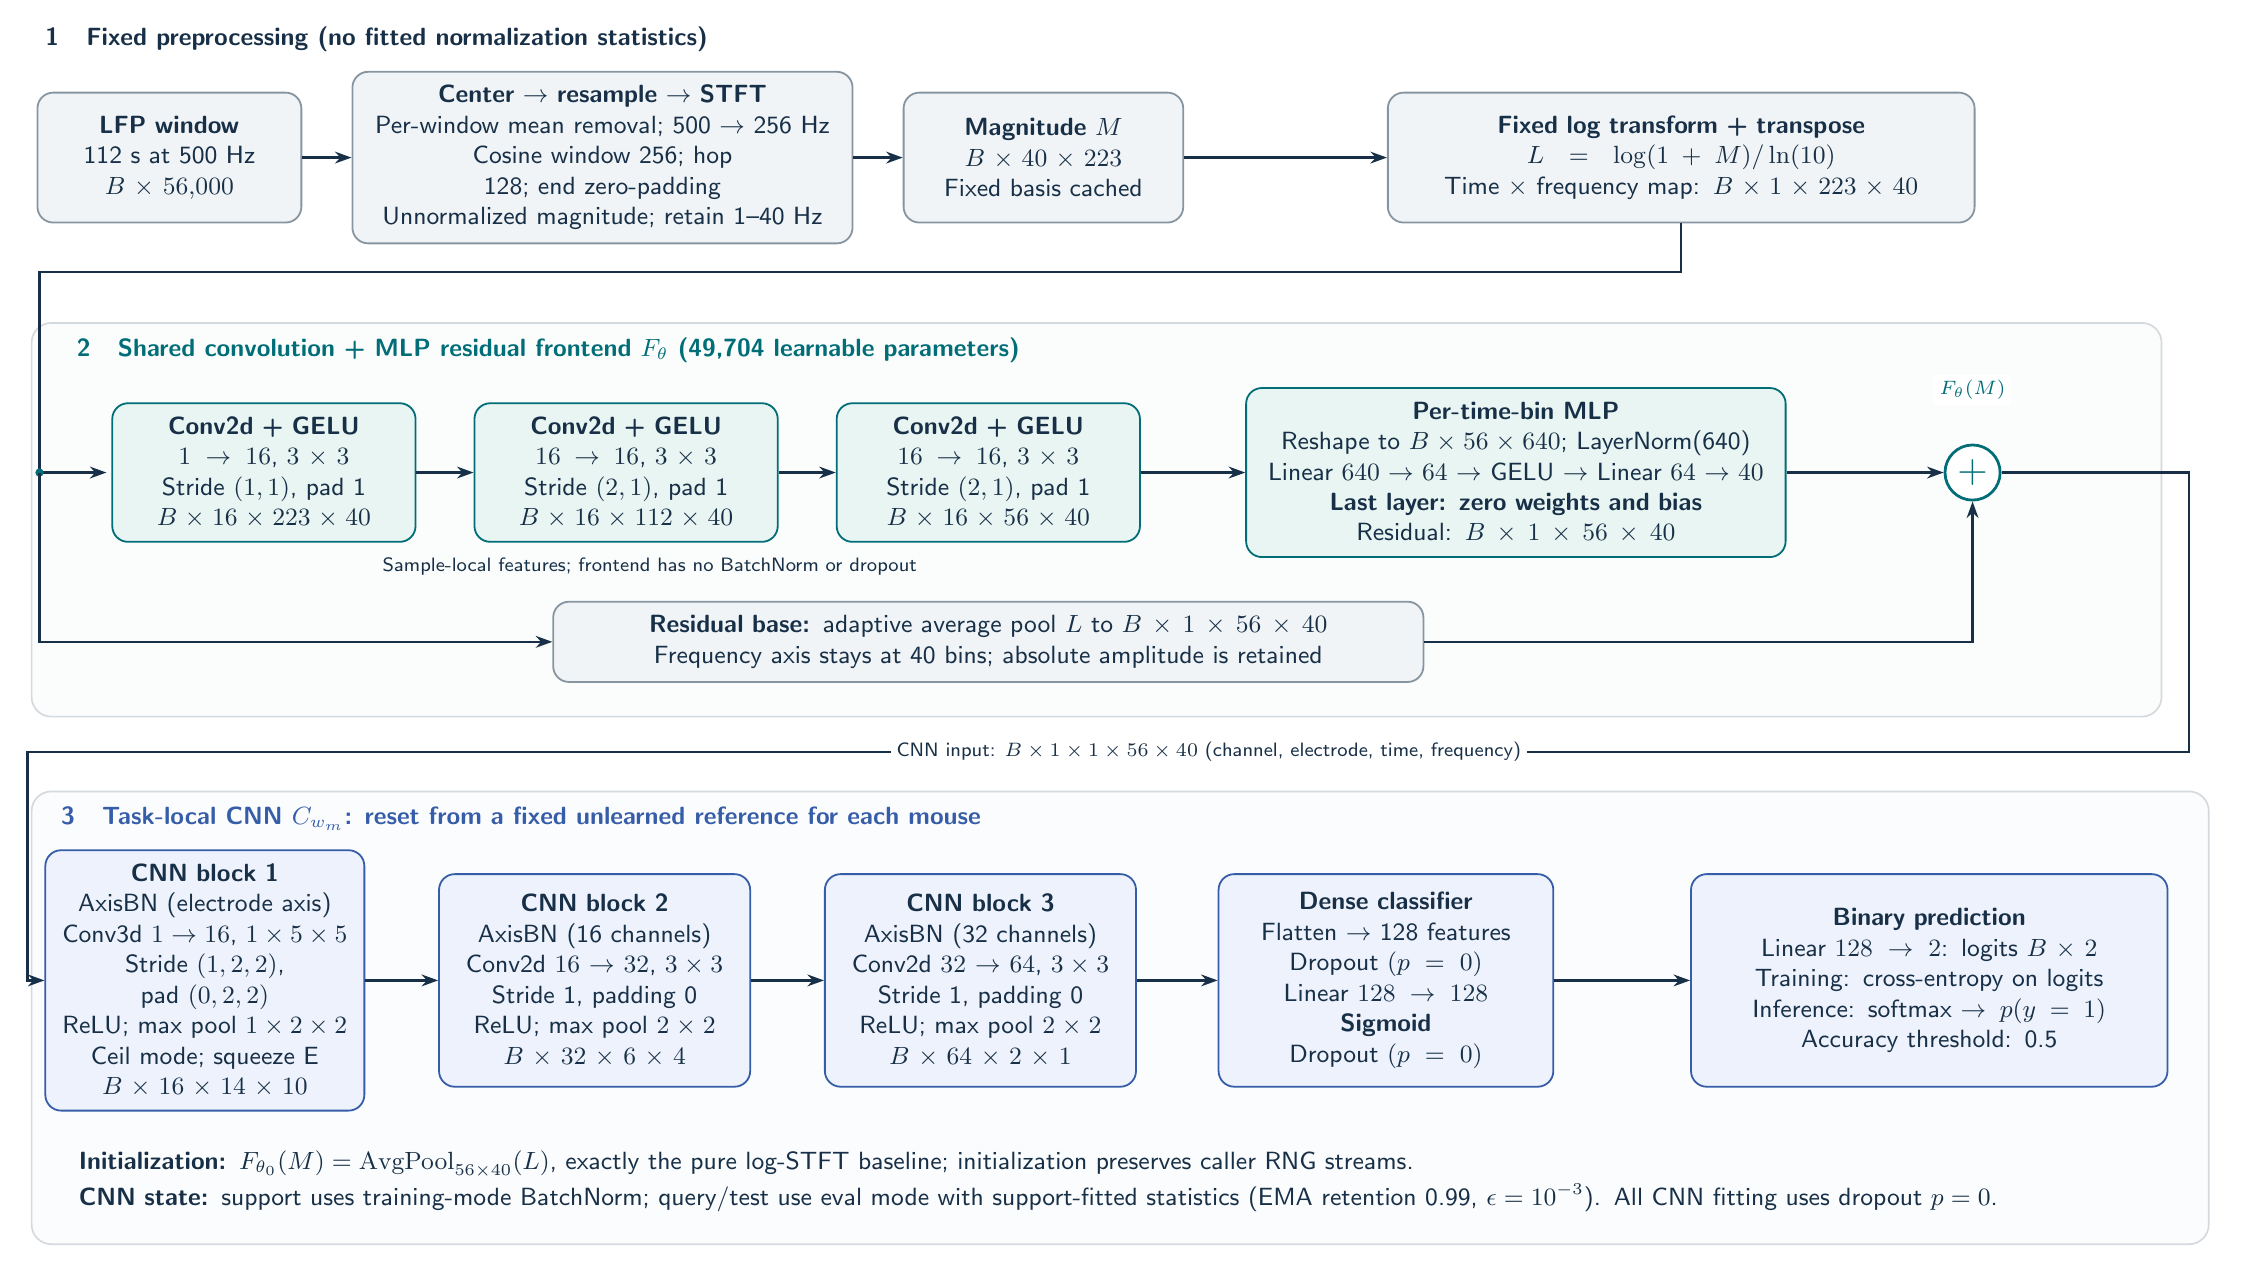
\begin{tikzpicture}[x=1cm,y=1cm]
\path[use as bounding box] (0,0) rectangle (27.8,15.6);

\node[section] at (0.1,15.45) {1\quad Fixed preprocessing (no fitted normalization statistics)};
\node[fixedbox,text width=3.0cm,minimum height=1.65cm] (raw) at (1.8,13.95)
  {\textbf{LFP window}\\112 s at 500 Hz\\\(B\times56{,}000\)};
\node[fixedbox,text width=6.0cm,minimum height=1.65cm] (prep) at (7.3,13.95)
  {\textbf{Center \(\to\) resample \(\to\) STFT}\\
   Per-window mean removal; 500 \(\to\) 256 Hz\\
   Cosine window 256; hop 128; end zero-padding\\
   Unnormalized magnitude; retain 1--40 Hz};
\node[fixedbox,text width=3.2cm,minimum height=1.65cm] (mag) at (12.9,13.95)
  {\textbf{Magnitude \(M\)}\\\(B\times40\times223\)\\Fixed basis cached};
\node[fixedbox,text width=7.1cm,minimum height=1.65cm] (log) at (21.0,13.95)
  {\textbf{Fixed log transform + transpose}\\
   \(L=\log(1+M)/\ln(10)\)\\
   Time \(\times\) frequency map: \(B\times1\times223\times40\)};
\draw[flow] (raw) -- (prep);
\draw[flow] (prep) -- (mag);
\draw[flow] (mag) -- (log);

\begin{scope}[on background layer]
  \draw[panel,fill=learnedbg!22] (0.05,6.85) rectangle (27.1,11.85);
  \draw[panel,fill=taskbg!22] (0.05,0.15) rectangle (27.7,5.9);
\end{scope}
\node[section,text=learned] at (0.5,11.5)
  {2\quad Shared convolution + MLP residual frontend \(F_\theta\) (49,704 learnable parameters)};

\coordinate (split) at (0.15,9.95);
\draw[flow] (log.south) -- (21.0,12.5) -- (0.15,12.5) -- (split) -- (1.0,9.95);
\fill[learned] (split) circle (1.5pt);
\node[learnedbox,text width=3.5cm,minimum height=1.75cm] (conv1) at (3.0,9.95)
  {\textbf{Conv2d + GELU}\\\(1\to16\), \(3\times3\)\\
   Stride \((1,1)\), pad 1\\\(B\times16\times223\times40\)};
\node[learnedbox,text width=3.5cm,minimum height=1.75cm] (conv2) at (7.6,9.95)
  {\textbf{Conv2d + GELU}\\\(16\to16\), \(3\times3\)\\
   Stride \((2,1)\), pad 1\\\(B\times16\times112\times40\)};
\node[learnedbox,text width=3.5cm,minimum height=1.75cm] (conv3) at (12.2,9.95)
  {\textbf{Conv2d + GELU}\\\(16\to16\), \(3\times3\)\\
   Stride \((2,1)\), pad 1\\\(B\times16\times56\times40\)};
\node[learnedbox,text width=6.5cm,minimum height=1.75cm] (mlp) at (18.9,9.95)
  {\textbf{Per-time-bin MLP}\\
   Reshape to \(B\times56\times640\); LayerNorm(640)\\
   Linear \(640\to64\) \(\to\) GELU \(\to\) Linear \(64\to40\)\\
   \textbf{Last layer: zero weights and bias}\\Residual: \(B\times1\times56\times40\)};
\node[circle,draw=learned,fill=white,line width=1pt,minimum size=7mm,inner sep=0pt,
  font=\Large,text=learned] (sum) at (24.7,9.95) {\(+\)};
\draw[flow] (conv1) -- (conv2);
\draw[flow] (conv2) -- (conv3);
\draw[flow] (conv3) -- (mlp);
\draw[flow] (mlp) -- (sum);

\node[fixedbox,text width=10.7cm,minimum height=0.9cm] (base) at (12.2,7.8)
  {\textbf{Residual base:} adaptive average pool \(L\) to \(B\times1\times56\times40\)\\
   Frequency axis stays at 40 bins; absolute amplitude is retained};
\draw[flow] (split) -- (0.15,7.8) -- (base.west);
\draw[flow] (base.east) -- (24.7,7.8) -- (sum.south);
\node[label,text=learned] at (24.7,11.0) {\(F_\theta(M)\)};
\node[label,fill=learnedbg!22] at (7.9,8.75)
  {Sample-local features; frontend has no BatchNorm or dropout};
\node[section,text=task] at (0.3,5.55)
  {3\quad Task-local CNN \(C_{w_m}\): reset from a fixed unlearned reference for each mouse};
\node[taskbox,text width=3.7cm,minimum height=2.7cm] (cnn1) at (2.25,3.5)
  {\textbf{CNN block 1}\\
   AxisBN (electrode axis)\\
   Conv3d \(1\to16\), \(1\times5\times5\)\\
   Stride \((1,2,2)\), pad \((0,2,2)\)\\
   ReLU; max pool \(1\times2\times2\)\\
   Ceil mode; squeeze E\\
   \(B\times16\times14\times10\)};
\node[taskbox,text width=3.6cm,minimum height=2.7cm] (cnn2) at (7.2,3.5)
  {\textbf{CNN block 2}\\
   AxisBN (16 channels)\\
   Conv2d \(16\to32\), \(3\times3\)\\
   Stride 1, padding 0\\
   ReLU; max pool \(2\times2\)\\
   \(B\times32\times6\times4\)};
\node[taskbox,text width=3.6cm,minimum height=2.7cm] (cnn3) at (12.1,3.5)
  {\textbf{CNN block 3}\\
   AxisBN (32 channels)\\
   Conv2d \(32\to64\), \(3\times3\)\\
   Stride 1, padding 0\\
   ReLU; max pool \(2\times2\)\\
   \(B\times64\times2\times1\)};
\node[taskbox,text width=3.9cm,minimum height=2.7cm] (dense) at (17.25,3.5)
  {\textbf{Dense classifier}\\
   Flatten \(\to\) 128 features\\Dropout \((p=0)\)\\
   Linear \(128\to128\)\\\textbf{Sigmoid}\\Dropout \((p=0)\)};
\node[taskbox,text width=5.7cm,minimum height=2.7cm] (output) at (24.15,3.5)
  {\textbf{Binary prediction}\\Linear \(128\to2\): logits \(B\times2\)\\
   Training: cross-entropy on logits\\
   Inference: softmax \(\to p(y=1)\)\\Accuracy threshold: 0.5};
\draw[flow] (sum.east) -- (27.45,9.95) -- (27.45,6.4) -- (0,6.4) -- (0,3.5) -- (cnn1.west);
\node[label] at (15.0,6.4)
  {CNN input: \(B\times1\times1\times56\times40\) (channel, electrode, time, frequency)};
\draw[flow] (cnn1) -- (cnn2);
\draw[flow] (cnn2) -- (cnn3);
\draw[flow] (cnn3) -- (dense);
\draw[flow] (dense) -- (output);
\node[align=left,text width=26.3cm,font=\small,text=ink] at (13.8,0.95)
  {\textbf{Initialization:} \(F_{\theta_0}(M)=\operatorname{AvgPool}_{56\times40}(L)\),
   exactly the pure log-STFT baseline; initialization preserves caller RNG streams.\\[2pt]
   \textbf{CNN state:} support uses training-mode BatchNorm; query/test use eval mode
   with support-fitted statistics (EMA retention 0.99, \(\epsilon=10^{-3}\)).
   All CNN fitting uses dropout \(p=0\).};
\end{tikzpicture}

\end{center}
\vfill
{\scriptsize\color{fixed}
  Implementation: \texttt{meta\_learning/frontend.py},
  \texttt{meta\_learning/model.py}, \texttt{models/cnn.py}.
  Teal: shared frontend parameters \(\theta\); blue: mouse-specific CNN parameters \(w_m\).
  Snapshot: 2026-10-16.}

\newpage
\heading{MouseLFP: frontend-only bilevel learning}{%
  One fixed task per configured mouse; support fits the CNN, query supervises the frontend,
  and test is inference only.}
\begin{center}
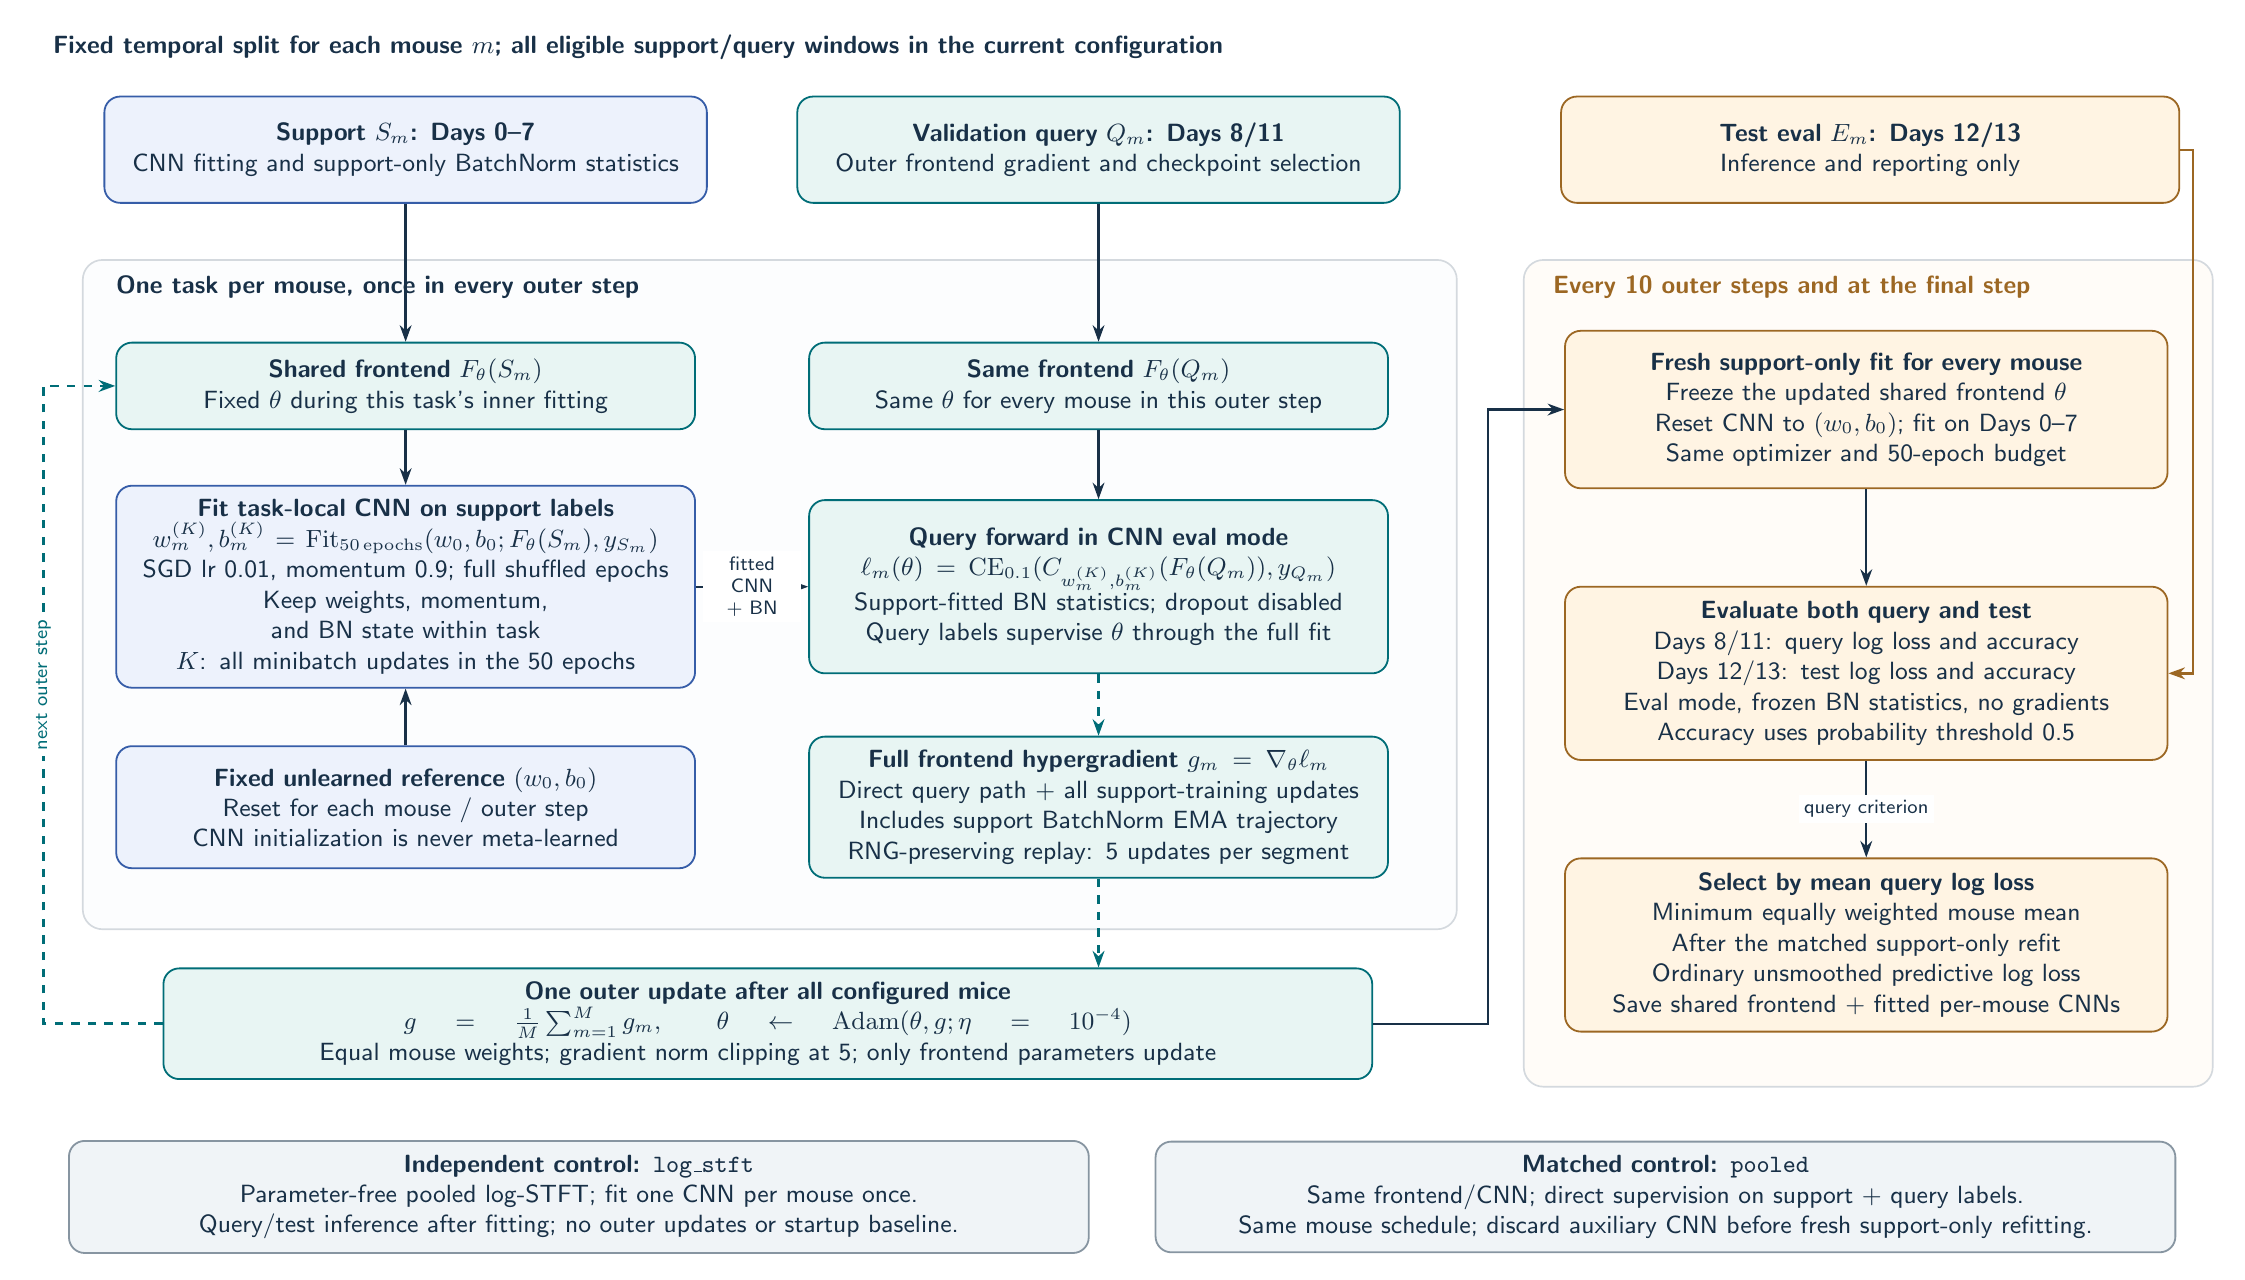
\begin{tikzpicture}[x=1cm,y=1cm]
\path[use as bounding box] (0,0) rectangle (27.8,15.55);
\node[section] at (0.2,15.3)
  {Fixed temporal split for each mouse \(m\); all eligible support/query windows in the current configuration};
\node[taskbox,text width=7.3cm,minimum height=1.35cm] (support) at (4.8,14.0)
  {\textbf{Support \(S_m\): Days 0--7}\\CNN fitting and support-only BatchNorm statistics};
\node[learnedbox,text width=7.3cm,minimum height=1.35cm] (query) at (13.6,14.0)
  {\textbf{Validation query \(Q_m\): Days 8/11}\\Outer frontend gradient and checkpoint selection};
\node[testbox,text width=7.5cm,minimum height=1.35cm] (test) at (23.4,14.0)
  {\textbf{Test eval \(E_m\): Days 12/13}\\Inference and reporting only};

\begin{scope}[on background layer]
  \draw[panel,fill=taskbg!18] (0.7,4.1) rectangle (18.15,12.6);
  \draw[panel,fill=heldoutbg!24] (19.0,2.1) rectangle (27.75,12.6);
\end{scope}
\node[section] at (1.0,12.25) {One task per mouse, once in every outer step};
\node[learnedbox,text width=7.0cm,minimum height=1.1cm] (sfeat) at (4.8,11.0)
  {\textbf{Shared frontend \(F_\theta(S_m)\)}\\Fixed \(\theta\) during this task's inner fitting};
\node[learnedbox,text width=7.0cm,minimum height=1.1cm] (qfeat) at (13.6,11.0)
  {\textbf{Same frontend \(F_\theta(Q_m)\)}\\Same \(\theta\) for every mouse in this outer step};
\draw[flow] (support) -- (sfeat);
\draw[flow] (query) -- (qfeat);

\node[taskbox,text width=7.0cm,minimum height=2.2cm] (fit) at (4.8,8.45)
  {\textbf{Fit task-local CNN on support labels}\\
   \(w_m^{(K)},b_m^{(K)}=\operatorname{Fit}_{50\,\mathrm{epochs}}
      (w_0,b_0;F_\theta(S_m),y_{S_m})\)\\
   SGD lr 0.01, momentum 0.9; full shuffled epochs\\
   Keep weights, momentum, and BN state within task\\
   \(K\): all minibatch updates in the 50 epochs};
\node[learnedbox,text width=7.0cm,minimum height=2.2cm] (qloss) at (13.6,8.45)
  {\textbf{Query forward in CNN eval mode}\\
   \(\ell_m(\theta)=\operatorname{CE}_{0.1}
     (C_{w_m^{(K)},b_m^{(K)}}(F_\theta(Q_m)),y_{Q_m})\)\\
   Support-fitted BN statistics; dropout disabled\\
   Query labels supervise \(\theta\) through the full fit};
\draw[flow] (sfeat) -- (fit);
\draw[flow] (qfeat) -- (qloss);
\draw[flow] (fit.east) -- node[label,text width=1.1cm] {fitted\\CNN + BN} (qloss.west);

\node[taskbox,text width=7.0cm,minimum height=1.55cm] (init) at (4.8,5.65)
  {\textbf{Fixed unlearned reference \((w_0,b_0)\)}\\
   Reset for each mouse / outer step\\
   CNN initialization is never meta-learned};
\draw[flow] (init) -- (fit);
\node[learnedbox,text width=7.0cm,minimum height=1.55cm] (grad) at (13.6,5.65)
  {\textbf{Full frontend hypergradient \(g_m=\nabla_\theta\ell_m\)}\\
   Direct query path + all support-training updates\\
   Includes support BatchNorm EMA trajectory\\
   RNG-preserving replay: 5 updates per segment};
\draw[gradient] (qloss) -- (grad);

\node[learnedbox,text width=15.0cm,minimum height=1.3cm] (update) at (9.4,2.9)
  {\textbf{One outer update after all configured mice}\\
   \(g=\frac{1}{M}\sum_{m=1}^{M}g_m,\qquad
     \theta\leftarrow\operatorname{Adam}(\theta,g;\eta=10^{-4})\)\\
   Equal mouse weights; gradient norm clipping at 5; only frontend parameters update};
\draw[gradient] (grad.south) -- (13.6,3.85) -- (update.north -| grad.south);
\draw[gradient] (update.west) -- (0.2,2.9) -- (0.2,11.0) -- (sfeat.west);
\node[label,rotate=90,text=learned] at (0.2,7.2) {next outer step};

\node[section,text=heldout] at (19.25,12.25) {Every 10 outer steps and at the final step};
\node[testbox,text width=7.3cm,minimum height=2.0cm] (refit) at (23.35,10.7)
  {\textbf{Fresh support-only fit for every mouse}\\
   Freeze the updated shared frontend \(\theta\)\\
   Reset CNN to \((w_0,b_0)\); fit on Days 0--7\\
   Same optimizer and 50-epoch budget};
\node[testbox,text width=7.3cm,minimum height=2.2cm] (score) at (23.35,7.35)
  {\textbf{Evaluate both query and test}\\
   Days 8/11: query log loss and accuracy\\
   Days 12/13: test log loss and accuracy\\
   Eval mode, frozen BN statistics, no gradients\\
   Accuracy uses probability threshold 0.5};
\node[testbox,text width=7.3cm,minimum height=2.2cm] (select) at (23.35,3.9)
  {\textbf{Select by mean query log loss}\\
   Minimum equally weighted mouse mean\\
   After the matched support-only refit\\
   Ordinary unsmoothed predictive log loss\\
   Save shared frontend + fitted per-mouse CNNs};
\draw[flow] (refit) -- (score);
\draw[flow] (score) -- node[label] {query criterion} (select);
\draw[flow,draw=heldout] (test.east) -- (27.5,14.0) -- (27.5,7.35) -- (score.east);
\draw[flow] (update.east) -- (18.55,2.9) -- (18.55,10.7) -- (refit.west);

\node[fixedbox,text width=12.6cm,minimum height=1.25cm] at (7.0,0.7)
  {\textbf{Independent control: \texttt{log\_stft}}\\
   Parameter-free pooled log-STFT; fit one CNN per mouse once.\\
   Query/test inference after fitting; no outer updates or startup baseline.};
\node[fixedbox,text width=12.6cm,minimum height=1.25cm] at (20.8,0.7)
  {\textbf{Matched control: \texttt{pooled}}\\
   Same frontend/CNN; direct supervision on support + query labels.\\
   Same mouse schedule; discard auxiliary CNN before fresh support-only refitting.};
\end{tikzpicture}

\end{center}
\vfill
{\scriptsize\color{fixed}
  Current \texttt{configs/meta.json}: targets=[X2], \(M=1\), 1,000 outer steps,
  batch size 32, 50 inner epochs, fixed shuffle seed 0, label smoothing 0.1.
  Full cohort: X1/X2/X4/X9/X10/X14/X15 (\(M=7\)).}

\newpage
\heading{MouseLFP: inner optimization unrolled as a recurrent graph}{%
  One mouse, one outer step. The recurrent state is the CNN, momentum, and BatchNorm state;
  each transition consumes one support minibatch.}
\begin{center}
% Forward dependencies and reverse-mode adjoints of one complete inner fit.
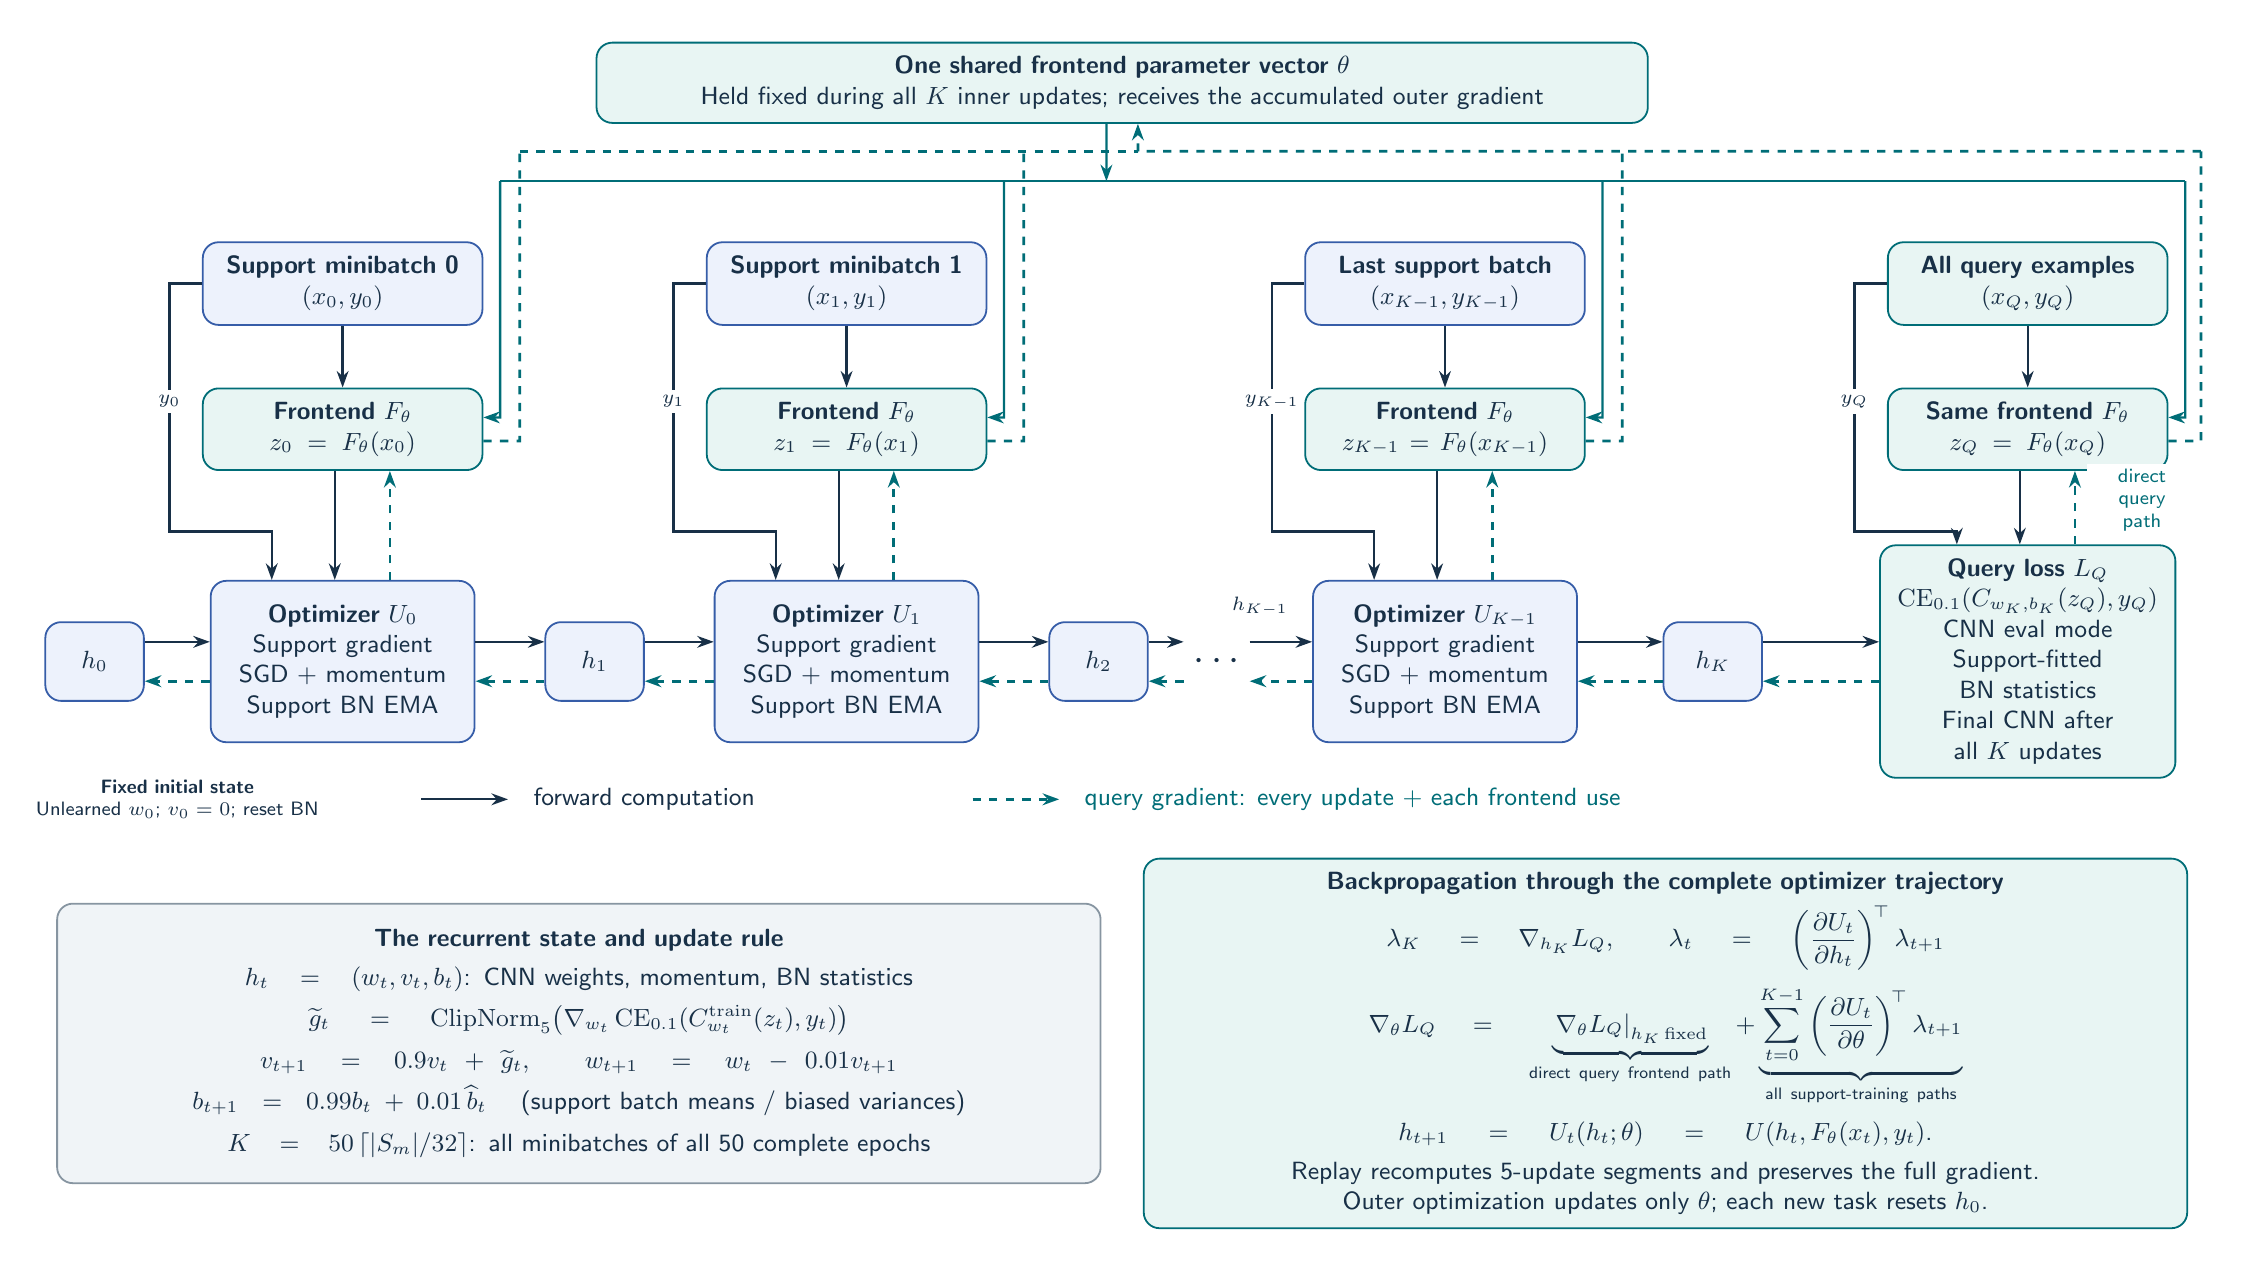
\begin{tikzpicture}[x=1cm,y=1cm]
\path[use as bounding box] (0,0) rectangle (27.8,15.55);

\node[learnedbox,text width=13.0cm,minimum height=0.85cm] (theta) at (13.9,14.85)
  {\textbf{One shared frontend parameter vector \(\theta\)}\\
   Held fixed during all \(K\) inner updates; receives the accumulated outer gradient};

% Support examples and the query branch are distinct inputs.
\node[taskbox,text width=3.2cm,minimum height=1.05cm] (batch0) at (4.0,12.3)
  {\textbf{Support minibatch 0}\\\((x_0,y_0)\)};
\node[taskbox,text width=3.2cm,minimum height=1.05cm] (batch1) at (10.4,12.3)
  {\textbf{Support minibatch 1}\\\((x_1,y_1)\)};
\node[taskbox,text width=3.2cm,minimum height=1.05cm] (batchlast) at (18.0,12.3)
  {\textbf{Last support batch}\\\((x_{K-1},y_{K-1})\)};
\node[learnedbox,text width=3.2cm,minimum height=1.05cm] (querydata) at (25.4,12.3)
  {\textbf{All query examples}\\\((x_Q,y_Q)\)};

\node[learnedbox,text width=3.2cm,minimum height=0.95cm] (front0) at (4.0,10.45)
  {\textbf{Frontend \(F_\theta\)}\\\(z_0=F_\theta(x_0)\)};
\node[learnedbox,text width=3.2cm,minimum height=0.95cm] (front1) at (10.4,10.45)
  {\textbf{Frontend \(F_\theta\)}\\\(z_1=F_\theta(x_1)\)};
\node[learnedbox,text width=3.2cm,minimum height=0.95cm] (frontlast) at (18.0,10.45)
  {\textbf{Frontend \(F_\theta\)}\\\(z_{K-1}=F_\theta(x_{K-1})\)};
\node[learnedbox,text width=3.2cm,minimum height=0.95cm] (frontq) at (25.4,10.45)
  {\textbf{Same frontend \(F_\theta\)}\\\(z_Q=F_\theta(x_Q)\)};
\foreach \a/\b in {batch0/front0,batch1/front1,batchlast/frontlast,querydata/frontq}
  \draw[flow] (\a.south) -- (\b.north);

% Shared-parameter broadcast; parallel dashed routes collect its adjoints.
\draw[flow,draw=learned] ([xshift=-2mm]theta.south) -- (13.7,13.6);
\draw[draw=learned,line width=0.85pt] (6.0,13.6) -- (27.4,13.6);
\draw[gradient] (27.6,13.98) -- (14.1,13.98) -- ([xshift=2mm]theta.south);
\draw[draw=learned,dashed,line width=1pt] (6.25,13.98) -- (14.1,13.98);
\foreach \front/\lane/\reverse in
  {front0/6.0/6.25,front1/12.4/12.65,frontlast/20.0/20.25,frontq/27.4/27.6} {
  \draw[flow,draw=learned] (\lane,13.6) -- (\lane,10.6) -- ([yshift=1.5mm]\front.east);
  \draw[draw=learned,dashed,line width=1pt]
    ([yshift=-1.5mm]\front.east) -- (\reverse,10.3) -- (\reverse,13.98);
}

\node[taskbox,text width=0.9cm,minimum height=1.0cm] (h0) at (0.85,7.5) {\(h_0\)};
\node[taskbox,text width=3.0cm,minimum height=2.05cm] (u0) at (4.0,7.5)
  {\textbf{Optimizer \(U_0\)}\\Support gradient\\
   SGD + momentum\\Support BN EMA};
\node[taskbox,text width=0.9cm,minimum height=1.0cm] (h1) at (7.2,7.5) {\(h_1\)};
\node[taskbox,text width=3.0cm,minimum height=2.05cm] (u1) at (10.4,7.5)
  {\textbf{Optimizer \(U_1\)}\\Support gradient\\
   SGD + momentum\\Support BN EMA};
\node[taskbox,text width=0.9cm,minimum height=1.0cm] (h2) at (13.6,7.5) {\(h_2\)};
\node[minimum width=0.7cm,minimum height=1.0cm,font=\Large,text=ink] (dots) at (15.1,7.5) {\(\cdots\)};
\node[taskbox,text width=3.0cm,minimum height=2.05cm] (ulast) at (18.0,7.5)
  {\textbf{Optimizer \(U_{K-1}\)}\\Support gradient\\
   SGD + momentum\\Support BN EMA};
\node[taskbox,text width=0.9cm,minimum height=1.0cm] (hk) at (21.4,7.5) {\(h_K\)};
\node[learnedbox,text width=3.4cm,minimum height=2.05cm] (loss) at (25.4,7.5)
  {\textbf{Query loss \(L_Q\)}\\
   \(\operatorname{CE}_{0.1}(C_{w_K,b_K}(z_Q),y_Q)\)\\
   CNN eval mode\\Support-fitted BN statistics\\Final CNN after all \(K\) updates};

% Forward state evolution and reverse query adjoints run in opposite directions.
\foreach \a/\b in {h0/u0,u0/h1,h1/u1,u1/h2,h2/dots,dots/ulast,ulast/hk,hk/loss} {
  \draw[flow] ([yshift=2.5mm]\a.east) -- ([yshift=2.5mm]\b.west);
  \draw[gradient] ([yshift=-2.5mm]\b.west) -- ([yshift=-2.5mm]\a.east);
}

% Feature inputs and their hypergradients; labels bypass the frontend.
\foreach \front/\cell/\batch/\labelx in
  {front0/u0/batch0/1.8,front1/u1/batch1/8.2,frontlast/ulast/batchlast/15.8,frontq/loss/querydata/23.2} {
  \draw[flow] ([xshift=-1mm]\front.south) -- ([xshift=-1mm]\cell.north);
  \draw[gradient] ([xshift=6mm]\cell.north) -- ([xshift=6mm]\front.south);
  \draw[flow] (\batch.west) -- (\labelx,12.3) -- (\labelx,9.15)
    -- ([xshift=-9mm]\cell.north |- 0,9.15) -- ([xshift=-9mm]\cell.north);
}
\node[label] at (1.8,10.8) {\(y_0\)};
\node[label] at (8.2,10.8) {\(y_1\)};
\node[label] at (15.8,10.8) {\(y_{K-1}\)};
\node[label] at (23.2,10.8) {\(y_Q\)};
\node[label,text=learned,anchor=west,text width=1.25cm] at (26.15,9.55) {direct query\\path};
\node[label] at (15.65,8.2) {\(h_{K-1}\)};

\node[align=center,font=\scriptsize,text=ink,text width=3.6cm] at (1.9,5.75)
  {\textbf{Fixed initial state}\\Unlearned \(w_0\); \(v_0=0\); reset BN};
\draw[flow] (5.0,5.75) -- (6.1,5.75);
\node[anchor=west,font=\small,text=ink] at (6.3,5.75) {forward computation};
\draw[gradient] (12.0,5.75) -- (13.1,5.75);
\node[anchor=west,font=\small,text=learned] at (13.3,5.75)
  {query gradient: every update + each frontend use};

\node[fixedbox,text width=12.9cm,minimum height=3.55cm] at (7.0,2.65)
  {\textbf{The recurrent state and update rule}\\[3pt]
   \(h_t=(w_t,v_t,b_t)\): CNN weights, momentum, BN statistics\\[4pt]
   \(\widetilde g_t=\operatorname{ClipNorm}_{5}
      \bigl(\nabla_{w_t}\operatorname{CE}_{0.1}(C^{\mathrm{train}}_{w_t}(z_t),y_t)\bigr)\)\\[4pt]
   \(v_{t+1}=0.9v_t+\widetilde g_t,\qquad w_{t+1}=w_t-0.01v_{t+1}\)\\[4pt]
   \(b_{t+1}=0.99b_t+0.01\,\widehat b_t\)
   \quad(support batch means / biased variances)\\[4pt]
   \(K=50\,\lceil |S_m|/32\rceil\): all minibatches of all 50 complete epochs};
\node[learnedbox,text width=12.9cm,minimum height=3.55cm] at (20.8,2.65)
  {\textbf{Backpropagation through the complete optimizer trajectory}\\[3pt]
   \(\lambda_K=\nabla_{h_K}L_Q,\qquad
      \lambda_t=\left(\dfrac{\partial U_t}{\partial h_t}\right)^{\!\top}\lambda_{t+1}\)\\[5pt]
   \(\displaystyle\nabla_\theta L_Q=
      \underbrace{\left.\nabla_\theta L_Q\right|_{h_K\,\mathrm{fixed}}}_{\text{direct query frontend path}}
      +\underbrace{\sum_{t=0}^{K-1}
       \left(\frac{\partial U_t}{\partial\theta}\right)^{\!\top}\lambda_{t+1}}_{\text{all support-training paths}}\)\\[5pt]
   \(h_{t+1}=U_t(h_t;\theta)=U(h_t,F_\theta(x_t),y_t)\).\\[3pt]
   Replay recomputes 5-update segments and preserves the full gradient.\\
   Outer optimization updates only \(\theta\); each new task resets \(h_0\).};
\end{tikzpicture}

\end{center}
\vfill
{\scriptsize\color{fixed}
  Support: Days 0--7. Query: Days 8/11. All intermediate updates represented by the ellipsis
  participate in backpropagation. Test Days 12/13 are inference only.
  Implementation: \texttt{meta\_learning/inner.py} and \texttt{meta\_learning/algorithms.py}.}
\end{document}
